\documentclass[11pt]{report}
\usepackage{titlesec}
\titleformat{\chapter}
  {\normalfont\LARGE\bfseries}{\thechapter}{1em}{}
\titlespacing*{\chapter}{0pt}{3.5ex plus 1ex minus .2ex}{2.3ex plus .2ex}

\usepackage{tabularx}
\usepackage[margin=1.2in]{geometry}
\usepackage[toc,page]{appendix}
\usepackage{graphicx}
\usepackage{lipsum}
\usepackage{booktabs}
\usepackage{caption}
\usepackage{forest}
\usepackage{tikz}
\usepackage{float}
\usetikzlibrary{trees, shapes.geometric, arrows, positioning}
\usepackage[utf8]{inputenc}
\usepackage[italian]{babel}
\usepackage{verbatim}
%\usepackage{colorprofiles}
\usepackage{listings}   %<- per inserire il codice
\usepackage{subcaption}
\usepackage{amsmath}
\usepackage{amsfonts}
\usepackage{longtable}
\usepackage{xcolor}
\usepackage{tcolorbox} % Gestisce i riquadri colorati

\newenvironment{notabox}
{\begin{tcolorbox}[colback=gray!10, colframe=black!70, title=Nota, fonttitle=\bfseries]}
{\end{tcolorbox}}

\lstset{
    basicstyle=\ttfamily\normalsize ,
    breaklines=true,
    moredelim=[is][\color{red}\itshape]{|R|}{|R|}
}

%%%%%%%%%%%%%%%%%%%%%%%%%%%%%%%%%%%%%%%%%%%%%%%%%%%%%%%%%%%%%%%%%%%%
\definecolor{custom_green}{rgb}{0,0.6,0}
\definecolor{codegray}{rgb}{0.5,0.5,0.5}
\definecolor{codepurple}{rgb}{0.58,0,0.82}
\definecolor{backcolour}{rgb}{0.95,0.95,0.92}
\definecolor{custom_blue}{rgb}{  0.05, 0.05, 0.97}
\definecolor{custom_brown}{rgb}{ 0.69, 0.38, 0.10}
\definecolor{custom_purple}{rgb}{0.58, 0.00, 0.82}
\definecolor{custom_orange}{rgb}{0.94, 0.59, 0.09}

\lstdefinestyle{MATLABstyle}{   
    commentstyle=\color{custom_green},
    keywordstyle=\color{magenta},
    numberstyle=\tiny\color{codegray},
    stringstyle=\color{codepurple},
    basicstyle=\ttfamily\footnotesize,
    breakatwhitespace=false,         
    breaklines=true,                 
    captionpos=b,                    
    keepspaces=true,                 
    numbers=left,                    
    numbersep=5pt,                  
    showspaces=false,                
    showstringspaces=false,
    showtabs=false,                  
    tabsize=2
}
\lstdefinelanguage{Cpp}{
      language=C++,
      backgroundcolor=\color{white},  
      basicstyle=\footnotesize \ttfamily \color{black} \bfseries,   
      breakatwhitespace=false,       
      breaklines=true,               
      captionpos=b,                   
      commentstyle=\color{custom_green},   
      deletekeywords={...},          
      escapeinside={\%*}{*)},
      keywordstyle=\color{custom_purple},
      identifierstyle=\color{blue},
      stringstyle=\color{blue},      
      numbers=left,                 
      numbersep=5pt,                  
      numberstyle=\tiny\color{black}, 
      rulecolor=\color{black},        
      showspaces=false,               
      showstringspaces=false,        
      showtabs=false,                
      stepnumber=1,                   
      tabsize=5,                     
      title=\lstname,                 
    }

\lstdefinelanguage{Python}{
    keywords={from, import, def, return, as, in, len, if, elif, else, for, while},
    breakatwhitespace=false,       
    breaklines=true,   
    morecomment=[l]{\#},
    morestring=[b]",
    commentstyle=\color{red},
    keywordstyle=\color{custom_purple},
    numberstyle=\tiny\color{black},
    stringstyle=\color{custom_green},
    basicstyle=\ttfamily\footnotesize,
    captionpos=b,
    showstringspaces=false,        
    showtabs=false,                
    numbers=left,                 
    numbersep=5pt,                  
    numberstyle=\tiny\color{black}, 
    rulecolor=\color{black},                      
    tabsize=5,                     
    title=\lstname,    
}

\lstdefinelanguage{MATLABc}{
    language=MATLAB,
    backgroundcolor=\color{white},  
    basicstyle=\footnotesize \ttfamily \color{black} \bfseries,   
    breakatwhitespace=false,       
    breaklines=true,               
    captionpos=b,
    morestring=[b]",
    commentstyle=\color{custom_green},   
    keywordstyle=\color{custom_blue},
    morekeywords={clearvars},
    deletekeywords={fprintf},
    identifierstyle=\color{black},
    stringstyle=\color{custom_purple},      
    numbers=left,                 
    numbersep=5pt,                  
    numberstyle=\tiny\color{black}, 
    rulecolor=\color{black},        
    showspaces=false,               
    showstringspaces=false,        
    showtabs=false,                
    stepnumber=1,                   
    tabsize=5,                     
    title=\lstname,                 
}

\lstdefinestyle{pythonstyle}{
    language=Python
}

\lstdefinestyle{promptstyle}{
    basicstyle=\ttfamily\small,
    breaklines=true,
    frame=single,
    backgroundcolor=\color{lightgray!20}, % Se hai il pacchetto xcolor attivo
    keywordstyle=\color{blue}
}
%%%%%%%%%%%%%%%%%%%%%%%%%%%%%%%%%%%%%%%%%%%%%%%%%%%%%%%%%%%%%%%%%%%%


\begin{document}
\nocite{*}
\captionsetup[figure]{margin=1.5cm,font=small,labelfont={bf},name={Figure},labelsep=colon,textfont={it}}
\captionsetup[table]{margin=1.5cm,font=small,labelfont={bf},name={Table},labelsep=colon,textfont={it}}


\begin{titlepage}
\begin{center}
\LARGE {\scshape{Università Politecnica delle Marche}}\\[0.5cm]
\LARGE {\scshape{Ingegneria Informatica e dell'Automazione}}\\[0.7cm]
\linespread{1}
\huge {\bfseries Emotion-Aware : Meta-Prompting for Marble 3D World Generation }\\[1cm]
\linespread{1}

\includegraphics[width=5cm]{images/logoUnivpm.jpg}\\[0.5cm]
\linespread{1.2}
\Large Corso di\\
\Large {\scshape{COMPUTER VISION E DEEP LEARNING}} \\[0.3cm]
\Large {Anno accademico 2025-2026 \\[0.8cm]}
{\Large Studenti:}
\hfill {\Large Professore:}\\
{\Large TOYEM TEZEM RYAN PARFAIT}
\hfill
{\Large ALESSANDRO GALDELLI}\\
\raggedright{\Large AGOSTINELLI SIMONE}
\hfill{\Large LORENZO STACCHIO}\\
\hfill 
{\Large ANDREA UBALDI}\\

\paragraph{}
\paragraph{}
\centering{

\includegraphics[width=2cm]{images/dii_new.png}\\[0.3cm]
\large Dipartimento di Ingegneria dell'Informazione\\[0.3cm]
}
\end{center}
\end{titlepage}

\pagenumbering{arabic}
\tableofcontents
\addcontentsline{toc}{chapter}{Introduzione}
\newpage

\pagestyle{plain}


\chapter*{Introduzione}
\addcontentsline{toc}{chapter}{Introduzione}
 
Questo progetto nasce come \textit{``A Self-Looping Reasoning Process for Simulating Human Behaviour''}, con l'idea di costruire un ciclo cognitivo chiuso basato su LLM, stati interni artificiali e aggiornamento iterativo del prompt. In questa versione rimodulata, il focus cambia: non si simula più il comportamento umano in TribeV2, ma si usa il progetto Liminal come base per generare prompt testuali destinati a Marble 3D World Generation.
 
Il sistema è un \textbf{meta-prompt generator emotion-aware}: riceve lo stimolo visivo osservato dall'utente, i dati emotivi e il messaggio testuale dell'utente; poi produce un prompt dettagliato per creare un mondo 3D in Marble capace di stimolare l'emotività e ridirezionare il pensiero dell'utente verso uno \textit\textbf{{stato liminal}}.
 
L'obiettivo è di realizzare una pipeline capace di trasformare emozioni e contenuti conversazionali in ambienti 3D generativi, nei quali la scena non sia solo coerente con lo stato emotivo dell'utente, ma sia anche progettata per guidare la riflessione verso il punto cardinale della conversazione.
 
Il presente rapporto è strutturato in cinque capitoli: il Capitolo~\ref{ch:fondazioni} presenta le fondazioni teoriche e l'architettura del sistema; il Capitolo~\ref{ch:sviluppo} dettaglia lo sviluppo di ogni fase della pipeline; il Capitolo~\ref{ch:problemi} documenta i problemi critici e le soluzioni adottate; il Capitolo~\ref{ch:risultati} analizza i risultati; il Capitolo~\ref{ch:conclusione} conclude con i limiti e le prospettive future.
 
% ── Diagramma architettura generale ──
\begin{figure}[H]
\centering
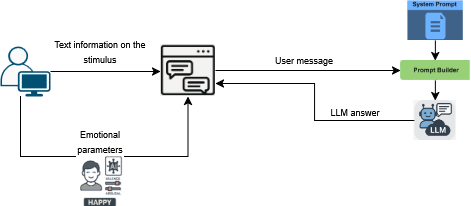
\includegraphics[width=1.0\textwidth,keepaspectratio]{images/diagram_projet.png}
\caption{Presentazione globale del progetto}
\label{fig:projet}
\end{figure}
 
 
% ═══════════════════════════════════════════════════════════════════
%              CAPITOLO I - FONDAZIONI TEORICHE E ARCHITETTURA
% ═══════════════════════════════════════════════════════════════════
\chapter{Fondazioni teoriche e architettura}
\label{ch:fondazioni}
 
% ─────────────── I.1 CADRE THÉORIQUE ───────────────
\section{Quadro teorico}
 
\subsection{Il concetto di spazio Liminal}
 
Il concetto di \textit{liminalità} descrive le fasi di transizione nella vita umana: momenti di ambiguità in cui l'ordine si dissolve e si apre uno spazio fluido, permettendo l'emergere di nuove idee, pratiche e identità. Lo stato Liminal propone un nuovo quadro di progettazione che va oltre la UX tradizionale (centrata su usabilità, piacere, efficienza) per creare esperienze che provocano \textbf{trascendenza e trasformazione personale}.
 
Il progetto mappa un percorso emotivo ben definito: lo stimolo visivo determina l'innesco di un'emozione (che in seguito sarà quantificata), mentre il messaggio dell'utente ne traccia la navigazione nello spazio intermedio. Questo spazio liminale trova la sua forma tangibile nel mondo Marble, un ambiente 3D ingegnerizzato per focalizzarsi sulla trasformazione emotiva, escludendo qualsiasi intento di distrazione o superficiale compiacimento.
 
\subsection{Concetti emozionali chiave}
 
\begin{itemize}
    \item[\textbf{Priming:}] Traccia emotiva indotta dallo stimolo visivo. Anche se l'utente ora appare neutro, il priming può continuare a influenzare la generazione del prompt.
    \item[\textbf{Realtime:}] Stato emotivo catturato dal volto dell'utente immediatamente dopo lo stimolo, prima della reazione testuale.
    \item[\textbf{Punto cardinale:}] La traiettoria evolutiva che guida la trasformazione emozionale, definita come passaggio dinamico dallo stato emotivo di partenza verso una direzione finale: non una semplice destinazione, ma un processo di ricondizionamento dell'emozione (dalla perdita verso la gratitudine, dalla diversità verso la connessione, dalla paura verso la protezione).
    \item[\textbf{Valenza:}]  Indicatore che categorizza l'emozione di partenza esclusivamente come positiva o negativa per impostare le condizioni iniziali del sistema.
    \item[\textbf{Arousal:}] Il livello di attivazione o eccitazione fisiologica indotto dallo stimolo (vagliato su una scala da $1$ a $10$). Rappresenta l'energia dell'emozione ed è indipendente dalla valenza (es. un'alta attivazione può indicare sia rabbia sia euforia).
    \item[\textbf{Intensità:}] La magnitudo o forza d'impatto con cui l'emozione si manifesta nel soggetto (scala $1$-$10$).
\end{itemize}
 
 
\subsection{Differenze rispetto al progetto originale}
 
\begin{table}[H]
    \centering
    \caption{Confronto tra la versione originale e la versione rimodulata del progetto.}
    \label{tab:confronto}
    \begin{tabularx}{\textwidth}{l X X}
        \toprule
        \textbf{Aspetto} & \textbf{Versione originale} & \textbf{Versione rimodulata} \\
        \midrule
        Obiettivo & Simulare stati mentali e comportamento umano in self-loop & Generare mondi 3D liminal per Marble \\
        Input & Scenario psicologico + LLM + feedback ambientale & Stimolo visivo + emozione rilevato + testo utente \\
        Output & Pensieri, azioni e comportamento simulato & Prompt Marble e mondo 3D \\
        Tecnologia & TribeV2 + reasoning LLM & Liminal + Llama + Marble \\
        Valutazione & Coerenza comportamentale & Coerenza emotiva + redirezione cognitiva \\
        \bottomrule
    \end{tabularx}
\end{table}
 
 
% ─────────────── I.2 ARCHITETTURA GLOBALE ───────────────
\section{Architettura globale del sistema}
 
\subsection{Schema generale}
 
La pipeline trasforma dati emozionali multimodali (priming facciale, emozione realtime, messaggio testuale) in un prompt narrativo per la generazione di mondi 3D in Marble, attraverso sette fasi sequenziali orchestrate da \texttt{pipeline.py}.
 
% ── Diagramma flusso pipeline ──

\begin{figure}[H]
\centering
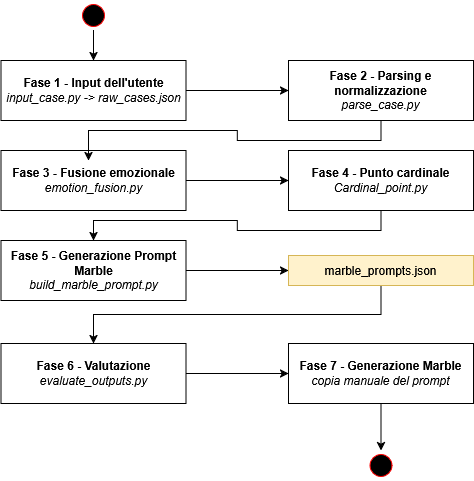
\includegraphics[width=0.55\textwidth,keepaspectratio]{images/diagramma di flusso.png}
\caption{Flusso completo della pipeline}
\label{fig:pipeline_flow}
\end{figure}
 
\subsection{Infrastruttura e comunicazione}
 
\begin{figure}[H]
\begin{verbatim}
progetto_d22_marble/
+-- data/
|   +-- raw_cases.json
|   +-- marble_prompts.json
|   +-- evaluation_report.json
|   +-- translations.json
+-- src/
|   +-- pipeline.py
|   +-- input_case.py
|   +-- parse_cases.py
|   +-- emotion_fusion.py
|   +-- cardinal_point.py
|   +-- build_marble_prompt.py
|   +-- evaluate_outputs.py
|   +-- config/
|   |   +-- emotions.py
|   |   +-- evualuate_expr.py
|   |   +-- patterns.py
|   +-- utils/
|   |   +-- file_utils.py
|   |   +-- spinner.py
|   |   +-- translator.py
|   +-- vpn_utils/
|       +-- ssh_con.py
|       +-- vpn.py
+-- prompts/
|   +-- meta_prompt_v2.txt
|   +-- emotion_text_analysis_prompt.txt
|   +-- cardinal_point_meta_prompt.txt
|   +-- emotion_alignment_prompt.txt
|   +-- cardinal_alignment_prompt.txt
+-- outputs/screenshots/
+-- .env
+-- requirements.txt
+-- README.md
\end{verbatim}
\caption{Organizzazione dei file del progetto.}
\end{figure}

Il sistema utilizza Ollama come server LLM, in due configurazioni possibili:
\begin{itemize}
    \item \textbf{Locale}: Llama3 (8B), chiamato direttamente su \texttt{localhost:11434}.
    \item \textbf{Remoto}: Qwen3 o Llama3 su server universitario (\texttt{192.168.80.138}), raggiungibile tramite VPN WireGuard + tunnel SSH con keepalive.
\end{itemize}
 
La selezione avviene tramite il file \texttt{.env} senza modificare il codice.

 
% ═══════════════════════════════════════════════════════════════════
%              CAPITOLO II - SVILUPPO DELLA PIPELINE
% ═══════════════════════════════════════════════════════════════════
\chapter{Sviluppo della pipeline}
\label{ch:sviluppo}
 
% ─────────────── II.1 INPUT ───────────────
\section{Fase 1: Input interattivo (\texttt{input\_case.py})}
 
\subsection{Interfaccia utente in italiano}
 
L'utente risponde a una serie di domande nel terminale in italiano. Il sistema supporta più emozioni per il priming (ciclo che termina con ``fine'') e traduce automaticamente le risposte in inglese per il formato JSON standardizzato.
 
\begin{figure}[H]
\begin{verbatim}
# Esempio di sessione
# > Quale stimolo visivo? Morte di Mufasa - Il Re Leone
# > Emozione priming? Felice
# > Intensita (1-10)? 8
# > Valenza (positiva/neutra/negativa)? positiva
# > Arousal (1-10)? 5
# > Messaggio? Mio padre e vivo e gli voglio bene!
\end{verbatim}
\caption{esempio di input utente.}
\end{figure}

\subsection{Traduzione e normalizzazione automatica}
 
La traduzione è gestita dal dizionario \texttt{data/translations.json}:
 
\begin{figure}[H]
\begin{verbatim}
{
  "emotions": {
    "felice": "Happy",
    "triste": "Sad",
    "arrabbiato": "Angry",
    "paura": "Fear"
  },
  "intensity": {
    "1": "LOW", "4": "MEDIUM", "8": "HIGH"
  },
  "valence": {
    "positiva": "POSITIVE",
    "neutra": "NEUTRAL",
    "negativa": "NEGATIVE"
  }
}
\end{verbatim}
\caption{esempio di traduzione dentro translations.json .}
\end{figure}
 
La probability è derivata automaticamente dall'intensità: $p = \frac{\text{intensity}}{10}$.
 
\subsection{Formato JSON standardizzato}
 
\begin{figure}[H]
\begin{verbatim}
{
  "case_id": "case_001",
  "timestamp": "2026-05-27T10:00:00",
  "stimulus": "Death of Mufasa - The Lion King",
  "priming_emotion": {
    "Happy": {
      "avg_intensity": "HIGH",
      "avg_arousal": "MEDIUM",
      "avg_valence": "POSITIVE",
      "emotion_probability": 0.80
    }
  },
  "realtime_face_emotion": {
    "dominant_emotion": "Happy",
    "probability": 0.90,
    "intensity_label": "HIGH",
    "valence_label": "POSITIVE",
    "arousal_label": "MEDIUM"
  },
  "user_message": "Sai che la morte di Mufasa non mi mette tristezza..."
}
\end{verbatim}
\caption{formato json di un caso standardizzato.}
\end{figure}
 
 
% ─────────────── II.2 PARSING ───────────────
\section{Fase 2: Parsing e normalizzazione (\texttt{parse\_cases.py})}
 
\subsection{Uniformizzazione delle etichette}
 
Il modulo legge \texttt{raw\_cases.json} e uniformizza tutte le etichette: ``happy'', ``felice'', ``felicità'' e ``gioia'' diventano tutti ``Happy''; ``ALTA'' diventa ``HIGH''; ``POSITIVA'' diventa ``POSITIVE''. Se un campo è assente, viene utilizzato un valore di default (intensity: ``MEDIUM'', probability: 0.5).
 
Questa fase è interamente in Python puro, senza nessuna chiamata di rete.
 
 
% ─────────────── II.3 FUSION ───────────────
\section{Fase 3: Fusione emozionale (\texttt{emotion\_fusion.py})}
 
\subsection{Tre segnali, tre pesi}
 
La fusione combina tre segnali con pesi definiti dal documento tecnico fornito dai tutor:
 
\begin{equation}
    S_\text{fusion}(e) = w_p \cdot S_\text{priming}(e) + w_r \cdot S_\text{realtime}(e) + w_t \cdot S_\text{testo}(e)
    \label{eq:fusion}
\end{equation}
 
dove $w_p = 0.35$, $w_r = 0.45$, $w_t = 0.20$ e $e$ è un'etichetta emozionale.
 
\begin{itemize}
    \item \textbf{Priming} ($\times 0.35$): $S_\text{priming}(e) = p_e \times I(e)$ dove $p_e$ è la probability e $I(e)$ il valore numerico dell'intensità.
    \item \textbf{Realtime} ($\times 0.45$): $S_\text{realtime}(e) = p_\text{dom} \times I_\text{dom}$ per l'emozione dominante.
    \item \textbf{Testo} ($\times 0.20$): classificazione emozionale del messaggio italiano tramite Llama (\textbf{Appello Llama \#1}).
\end{itemize}
 
La conversione delle etichette in valori numerici segue la tabella:
 
\begin{table}[H]
    \centering
    \caption{Mappatura delle etichette a valori numerici.}
    \label{tab:label_map}
    \begin{tabular}{lc|lc|lc}
        \toprule
        \textbf{Intensity} & \textbf{Valore} & \textbf{Valence} & \textbf{Valore} & \textbf{Arousal} & \textbf{Valore} \\
        \midrule
        HIGH & 1.0 & POSITIVE & +1.0 & HIGH & 1.0 \\
        MEDIUM & 0.6 & NEUTRAL & 0.0 & MEDIUM & 0.5 \\
        LOW & 0.3 & NEGATIVE & $-$1.0 & LOW & 0.2 \\
        \bottomrule
    \end{tabular}
\end{table}
 
\subsection{Analisi testuale via Llama}
 
Il messaggio italiano viene inviato direttamente a Llama con il prompt \texttt{emotion\_text\_analysis\_prompt.txt}. Llama legge il prompt e genera una risposta standard per l'elaborazione successiva. In caso di fallimento nella generazione della risposta si attiva una funzione di fallback statica, basata su keyword matching.
 
\subsection{Caso Mufasa: dimostrazione del calcolo}
 
Per il caso della morte di Mufasa, con messaggio \textit{``Sai che la morte di Mufasa non mi mette tristezza perché mio padre è vivo e gli voglio molto bene!''}:
 
\begin{align}
    S_\text{priming}(\text{Happy}) &= 0.60 \times 1.0 = 0.60 \nonumber \\
    S_\text{priming}(\text{Sad}) &= 0.20 \times 0.6 = 0.12 \nonumber \\[6pt]
    S_\text{realtime}(\text{Happy}) &= 0.95 \times 1.0 = 0.95 \nonumber \\[6pt]
    S_\text{testo}(\text{Sad}) &= 0.70 \quad (\text{Llama}) \nonumber \\
    S_\text{testo}(\text{Tenderness}) &= 0.40 \quad (\text{Llama}) \nonumber
\end{align}
 
Fusione:
\begin{align}
    F(\text{Happy}) &= 0.60 \times 0.35 + 0.95 \times 0.45 + 0 \times 0.20 = \mathbf{0.6375} \leftarrow \text{dominante} \nonumber \\
    F(\text{Sad}) &= 0.12 \times 0.35 + 0 \times 0.45 + 0.70 \times 0.20 = 0.182 \nonumber \\
    F(\text{Tenderness}) &= 0 \times 0.35 + 0 \times 0.45 + 0.40 \times 0.20 = 0.08 \nonumber
\end{align}
 
\subsection{Impatto del modello LLM sulla Pipeline}

La scelta del Large Language Model (LLM) si è rivelata un fattore discriminante e critico per la stabilità dell'intera architettura. Durante la fase di sviluppo e testing, l'impiego del modello compatto \texttt{Qwen3:1.7b} ha evidenziato forti limiti strutturali nelle capacità di ragionamento e di text-to-JSON. Di fronte alle richieste di analisi testuale e sentiment analysis, il modello falliva sistematicamente nel rispettare il vincolo sintattico richiesto, restituendo come output stringhe JSON vuote o degenerate (nello specifico, strutture formattate come \texttt{\{\textbackslash n\textbackslash n\textbackslash n\}}).

Questo comportamento ha messo in luce la vulnerabilità intrinseca di un'architettura sequenziale. L'assenza di dati strutturati validi a monte ha innescato un fenomeno di fallimento a cascata (\textit{cascade failure}): poiché i moduli successivi della pipeline (quali l'estrazione dei parametri affettivi e la successiva renderizzazione 3D nel mondo Marble) dipendono strettamente dal parsing dell'output dell'LLM, il blocco del primo nodo ha causato il degrado e l'arresto dell'intero flusso computazionale a valle.

A fronte di tale criticità, si è valutata l'adozione di un modello a più larga scala. Tuttavia, la versione di \texttt{Qwen} da 8 miliardi di parametri si è dimostrata eccessivamente onerosa in termini di allocazione di memoria e potenza computazionale; le risorse di calcolo universitarie a disposizione per il progetto non erano infatti sufficienti a garantirne l'esecuzione locale e l'inferenza in tempi accettabili. 

Per ovviare a questo vincolo infrastrutturale senza rinunciare alla precisione analitica, la scelta è ricaduta su \texttt{Llama3 (8B)}. A parità di ordine di grandezza dei parametri, questo modello ha offerto una migliore ottimizzazione delle risorse hardware disponibili, risolvendo completamente il collo di bottiglia strutturale. L'adozione di \texttt{Llama3 (8B)} ha garantito la corretta generazione di file JSON validi sia dal punto di vista sintattico che semantico, assicurando così la necessaria robustezza e continuità operativa a tutta la pipeline del progetto.
 
 
% ─────────────── II.4 CARDINAL POINT ───────────────
\section{Fase 4: Punto cardinale (\texttt{cardinal\_point.py})}
 
\subsection{Ruolo del punto cardinale nel quadro Liminal}

All'interno dell'architettura concettuale del progetto, il \textit{Punto Cardinale} non si configura come una mera etichetta categoriale, bensì come il principio regolatore e il vettore geometrico-emotivo che governa l'intero spazio liminale. Nel quadro di \textit{Liminal}, l'esperienza dell'utente non è statica, ma è definita da una transizione dinamica; in questo contesto, il punto cardinale assume il ruolo fondamentale di orientare questa traiettoria evolutiva.

A differenza dei sistemi tradizionali di computazione affettiva, che si limitano a fotografare e quantificare lo stato psicologico istantaneo del soggetto, il punto cardinale introduce una dimensione trasformativa. Esso opera integrando simultaneamente due coordinate fondamentali:
\begin{enumerate}
    \item \textbf{L'ancoraggio allo stato di partenza:} Il sistema riconosce e valida l'emozione iniziale (spesso a valenza negativa o ad alto arousal, come la paura o la tristezza), assumendola come punto di origine del vettore.
    \item \textbf{La direzione verso la meta costruttiva:} Il sistema identifica la polarità opposta o di risoluzione (come la protezione o la gratitudine), stabilendo la destinazione ideale dell'esperienza.
\end{enumerate}

Il Punto Cardinale agisce quindi come un vero e proprio ponte semantico tra l'analisi del testo (eseguita dall'LLM) e il motore di generazione procedurale dell'ambiente 3D. Esso traduce la complessa sfumatura emotiva del messaggio dell'utente in coordinate matematiche e scelte di design tangibili all'interno del mondo Marble. Parametrizzando la transizione (ad esempio, definendo il passaggio da \textit{perdita} a \textit{gratitudine}), il punto cardinale stabilisce le regole di mutamento della geometria, delle palette cromatiche e della densità degli asset nel mondo virtuale. 

In sintesi, nel quadro \textit{Liminal}, il punto cardinale è l'elemento software e concettuale che impedisce al sistema di essere un semplice specchio passivo del malessere dell'utente, trasformandolo invece in uno spazio attivo di accoglienza, elaborazione e trasformazione emotiva.
 
\subsection{Identificazione via Llama}
 
Il messaggio e l'emozione dominante vengono inviati a Llama (\textbf{Appello \#2}) con il prompt \texttt{cardinal\_point\_meta\_prompt.txt}. Llama restituisce:
\begin{itemize}
    \item \texttt{emotion\_target}: etichetta target validata contro l'enum \texttt{EmotionTarget} (Hope, Nostalgia, Acceptance, Connection, Gratitude, Joy, Safety, Tenderness, Neutral).
    \item \texttt{cardinal\_point}: direzione riflessiva (es.\ ``from loss toward gratitude'').
\end{itemize}
 
\subsection{Meccanismo di fallback}

Per garantire la robustezza e la tolleranza ai guasti (\textit{fault tolerance}) dell'intera architettura, è stato implementato un meccanismo di fallback deterministico. Nel caso in cui il modello \texttt{Llama3} dovesse fallire nell'inferenza, riscontrare problemi di latenza o restituire un'emozione non codificata (quindi non valida per il sistema), la pipeline non si interrompe, ma devia il flusso computazionale su una logica di riserva.

Questo modulo di salvataggio si appoggia alla tabella statica preconfigurata \texttt{EMOTION\_TO\_TARGET}. La tabella mappa in modo rigido le emozioni dell'utente in ingresso verso punti cardinali standard (es. from \texttt{Happy} toward \texttt{Gratitude}, from \texttt{Sad} toward \texttt{Hope}, from \texttt{Angry} toward \texttt{Acceptance}). Sebbene questo approccio escluda la granularità e la flessibilità dell'analisi semantica dinamica dell'LLM, assicura la continuità operativa del sistema, garantendo che il mondo \textit{Marble} riceva sempre un input strutturato valido per la generazione dell'ambiente 3D.

 
% ─────────────── II.5 BUILD MARBLE PROMPT ───────────────
\section{Fase 5: Generazione del prompt Marble (\texttt{build\_marble\_prompt.py})}
 
\subsection{Assemblaggio del prompt per Llama}
 
Il modulo carica \texttt{meta\_prompt\_v2.txt} e inietta i dati tramite \texttt{.replace()} (non \texttt{.format()}, per evitare conflitti con le parentesi graffe del JSON). Vengono iniettate nel prompt le seguenti variabili:
\begin{itemize}
    \item \textbf{stimulus:} La descrizione testuale dello stimolo visivo presentato all'utente.
    \item \textbf{priming\_emotion:} L'emozione teorica di partenza che lo stimolo mira a indurre nel soggetto.
    \item \textbf{realtime\_face\_emotion:} Lo stato emotivo dell'utente rilevato in tempo reale tramite computer vision ed espressioni facciali.
    \item \textbf{user\_message:} Il contenuto testuale del messaggio formulato dall'utente in risposta all'esperienza.
    \item \textbf{fusion\_profile:} Il profilo affettivo unificato ottenuto integrando i dati della face emotion e l'analisi semantica del testo.
    \item \textbf{emotion\_target:} La meta emotiva finale (la destinazione del punto cardinale) verso cui orientare la trasformazione del mondo 3D.
\end{itemize}

Infine, all'interno del meta-prompt viene iniettato anche il \texttt{cardinal\_hint}: una stringa di testo che racchiude il punto cardinale calcolato, fondamentale per guidare semanticamente l'LLM verso la corretta direzione di trasformazione.
 
\subsection{Il meta-prompt: cuore del sistema}
 
Il meta-prompt contiene la tabella di mappatura emozione $\rightarrow$ mondo 3D:
 
\begin{table}[H]
    \centering
    \caption{Mappatura emozione $\rightarrow$ elementi del mondo Marble.}
    \label{tab:emotion_world}
    \footnotesize
    \begin{tabularx}{\textwidth}{l X}
        \toprule
        \textbf{Emozione} & \textbf{Elementi del mondo 3D} \\
        \midrule
        Happy/Joy & Paesaggio aperto, giardino, savana, luce calda dorata, giallo/oro/arancio/verde \\
        Tenderness & Spazio protetto, luce soffusa, rosa/crema/azzurro, lanterne, cuscini, curve \\
        Sad & Paesaggio sospeso, lago, nebbia, luce fredda ma non oppressiva, blu/grigio/viola \\
        Fear & Spazio protetto in ambiente incerto, contrasti controllati, blu scuro/verde smorzato \\
        Anger & Paesaggio roccioso o metallico, luce dura ma trasformativa, rosso/arancio/rame \\
        Neutral & Spazio contemplativo minimale, luce naturale equilibrata, beige/grigio/azzurro pallido \\
        Surprise & Mondo rivelatorio, canyon, portale, luce dinamica, turchese/oro/viola \\
        Disgust & Ambiente di purificazione, luce fredda con zone pulite, verde scuro/grigio/bianco \\
        \bottomrule
    \end{tabularx}
\end{table}
 
Le \textit{transformation rules} definiscono la logica di risoluzione del sistema, specialmente in presenza di input discordanti: se lo stimolo iniziale induce tristezza ma il messaggio dell'utente esprime una reazione positiva, le regole non assecondano lo stato passivo del trigger, bensì ne governano il superamento. Il sistema adotta quindi la polarità positiva del testo come pivot, guidando la generazione verso la gratitudine (la meta corrispondente alla felicità espressa dall'utente) anziché appiattirsi sull'emozione negativa dello stimolo.
 
\subsection{Invocazione dell'LLM e Strategie di Parsing}

Il modulo di analisi testuale si affida a un'interazione strutturata con il modello \texttt{Llama3 (8B)}. Il sistema esegue una chiamata API configurata con parametri rigorosi, mirati a bilanciare la creatività semantica con la stabilità sintattica dell'output:
\begin{itemize}
    \item \texttt{format: json}: Vincola il modello a strutturare la risposta esclusivamente in formato JSON;
    \item \texttt{temperature: 0.7}: Regola il grado di libertà del modello, permettendo un'analisi semantica ricca senza compromettere l'aderenza alle istruzioni del prompt;
    \item \texttt{num\_predict: 2048}: Definisce la finestra massima di token generabili, garantendo lo spazio necessario per l'estrazione completa delle feature;
    \item \texttt{timeout: 180s}: Scongiura il blocco della pipeline in caso di latenza del server hardware.
\end{itemize}

Una volta ricevuto l'output, il sistema si scontra con la natura intrinsecamente stocastica degli LLM, i quali possono occasionalmente violare il formato richiesto. Per garantire la massima robustezza ed evitare fallimenti a cascata, il \textit{parser} è stato progettato come un sistema di difesa a quattro stadi sequenziali:

\begin{enumerate}
    \item \textbf{Pre-processing ed eliminazione del Markdown:} Il sistema applica espressioni regolari per rimuovere i blocchi di formattazione \verb|```json| e \verb|```| inseriti dall'LLM attorno al codice.
    \item \textbf{Parsing Diretto:} Si tenta l'immediata deserializzazione della stringa pulita tramite la libreria standard \texttt{json}.
    \item \textbf{Scansione dei blocchi nidificati:} In caso di fallimento, l'algoritmo analizza la stringa carattere per carattere calcolando la profondità delle parentesi graffe. Isola così i candidati JSON validi e seleziona la struttura più completa (prioritizzando la presenza della chiave \texttt{marble\_prompt}).
    \item \textbf{Estrazione Manuale (Fallback):} Qualora nessun blocco risulti sintatticamente valido, il sistema delega il recupero delle feature affettive a una funzione di estrazione euristica dal testo grezzo.
\end{enumerate}
 
\subsection{Esempio di output generato}
 
\begin{figure}[H]
\begin{verbatim}
{
  "runtime_analysis": {
    "dominant_emotion": "Happy",
    "complex_emotion": "Gratitude and familial affection",
    "cardinal_point": "From loss to presence and gratitude",
    "world_objective": "Amplify tenderness and emotional safety"
  },
  "marble_prompt": "Imagine a sunlit savannah at dawn, where
    golden grasses sway gently in the morning breeze...",
  "negative_constraints": [
    "No grief-focused imagery",
    "No darkness or cold tones",
    "No isolation or threatening elements"
  ],
  "variants": ["prompt alternativo 1...", "prompt alternativo 2..."]
}
\end{verbatim}
\caption{Prompt Marble generato per il caso Mufasa.}
\end{figure} 
 
% ─────────────── II.6 EVALUATION ───────────────
\section{Fase 6: Valutazione (\texttt{evaluate\_outputs.py})}

La fase finale del framework è deputata alla validazione del prompt generato, verificandone l'idoneità prima dell'effettivo inserimento all'interno del mondo \textit{Marble}. Il processo quantifica la qualità dell'output basandosi su cinque metriche fondamentali, ciascuna valutata su una scala Likert da $1$ a $5$:

\begin{itemize}
    \item \textbf{Emotion Alignment:} Valuta il grado di coerenza del prompt rispetto all'emozione target, verificando se le caratteristiche descritte comunichino efficacemente lo stato affettivo finale.
    \item \textbf{Cardinal Alignment:} Misura l'efficacia degli elementi comunicativi nel guidare e supportare la transizione psicologica ed evolutiva definita dal Punto Cardinale.
    \item \textbf{Prompt Concreteness:} Verifica la fattibilità tecnica dell'output, accertandosi che il prompt contenga asset, geometrie ed elementi concretamente renderizzabili in un ambiente 3D.
    \item \textbf{Prompt Diversity:} Monitora la variabilità del sistema, assicurando che l'output si difformi significativamente dalle generazioni precedenti associate a target emotivi differenti, scongiurando fenomeni di appiattimento stilistico.
    \item \textbf{Safety and Ethics:} Presidia i vincoli etici del progetto, garantendo che il modello eviti formulazioni di tipo diagnostico o clinico in merito alle emozioni dell'utente, limitando il proprio raggio d'azione alla sola descrizione oggettiva del mondo 3D.
\end{itemize}
 
\subsection{Approccio LLM-as-a-Judge}
 
Per automatizzare e rendere oggettivo il processo di valutazione descritto, si è adottato l'approccio \textit{LLM-as-a-Judge}, integrando il framework open-source \texttt{DeepEval}. Questa metodologia prevede l'utilizzo di un Large Language Model con il ruolo di valutatore indipendente degli output generati dalla pipeline; nello specifico, per mantenere l'intera architettura locale e limitare i costi, è stato impiegato il modello \texttt{Qwen3:1.7b}.

L'impiego di \texttt{Qwen3:1.7b} risponde non solo a vincoli di sostenibilità hardware locale, ma soddisfa una precisa scelta metodologica: la necessità di differenziare il modello generatore (\texttt{Llama3}) dal modello valutatore. Configurare due LLM distinti all'interno della pipeline permette di preservare l'indipendenza del giudizio, mitigando il fenomeno del \textit{self-correction bias} (o bias di auto-favoritismo). L'utilizzo del medesimo modello per entrambe le fasi avrebbe infatti introdotto il rischio latente di una sovrastima dei punteggi, dovuta alla parzialità intrinseca del modello verso le proprie strutture sintattiche e scelte stilistiche, inficiando così l'oggettività della validazione.

\subsubsection*{Utilizzo di DeepEval}
Inizialmente si è valutato l'impiego di \texttt{G-Eval}, una metrica standard di \texttt{DeepEval} basata su framework di valutazione generici. Tuttavia, i test preliminari con questo modello compatto hanno evidenziato una forte tendenza all'allucinazione nei punteggi numerici finali: il voto quantitativo (da $1$ a $5$) risultava spesso matematicamente incoerente con la motivazione testuale (\textit{reasoning}) prodotta dall'LLM stesso (ad esempio, a fronte di una critica severa nella motivazione veniva assegnato un punteggio massimo).

Per superare questo limite, si è optato per la creazione di una \textbf{metrica personalizzata} (\texttt{OllamaJudgeMetric}) all'interno del framework \texttt{DeepEval}. L'approccio si basa su un meta-prompt minimale e ottimizzato per le capacità computazionali del modello compatto, memorizzato nel file esterno \texttt{evaluator\_prompt.txt}. Per ciascuna delle cinque metriche, il sistema inietta dinamicamente nel template le informazioni verticali necessarie (i criteri specifici e i passaggi logici di validazione), strutturando la richiesta secondo lo schema seguente:

\begin{lstlisting}[style=promptstyle, caption={Contenuto di evaluator\_prompt.txt.}]
{criteria}

EVALUATION STEPS:
{steps_text}

INPUT: {input}
OUTPUT TO EVALUATE: {actual_output}

Respond ONLY with valid JSON:
{"score": value, "motivation": "explanation referencing... "}

Score must be one of: 0.0, 0.2, 0.4, 0.6, 0.8, 1.0
\end{lstlisting}

Questo condizionamento rigido e la richiesta di un output in formato JSON puro (vincolato a una scala discreta normata da $0.0$ a $1.0$) hanno costretto il modello a formalizzare il ragionamento (\textit{reasoning}) prima di emettere il verdetto. L'esplicitazione sequenziale degli \texttt{EVALUATION STEPS} ha così guidato la logica di \texttt{Qwen}, riducendo drasticamente le discrepanze tra la valutazione qualitativa espressa nella motivazione e il punteggio numerico finale.

 
% ─────────────── II.7 MARBLE ───────────────
\section{Fase 7: Generazione Marble e Risultati Visivi}

L'ultimo stadio della pipeline prevede l'effettiva materializzazione dell'ambiente tridimensionale. Il \texttt{marble\_prompt} generato dall'LLM viene copiato all'interno dell'interfaccia di \textit{Marble}. dopo che marble abbia generato il mondo viene fatto una cattura e inserito a mano dentro la cartella \texttt{outputs/screenshots/}.

\begin{figure}[H]
\centering
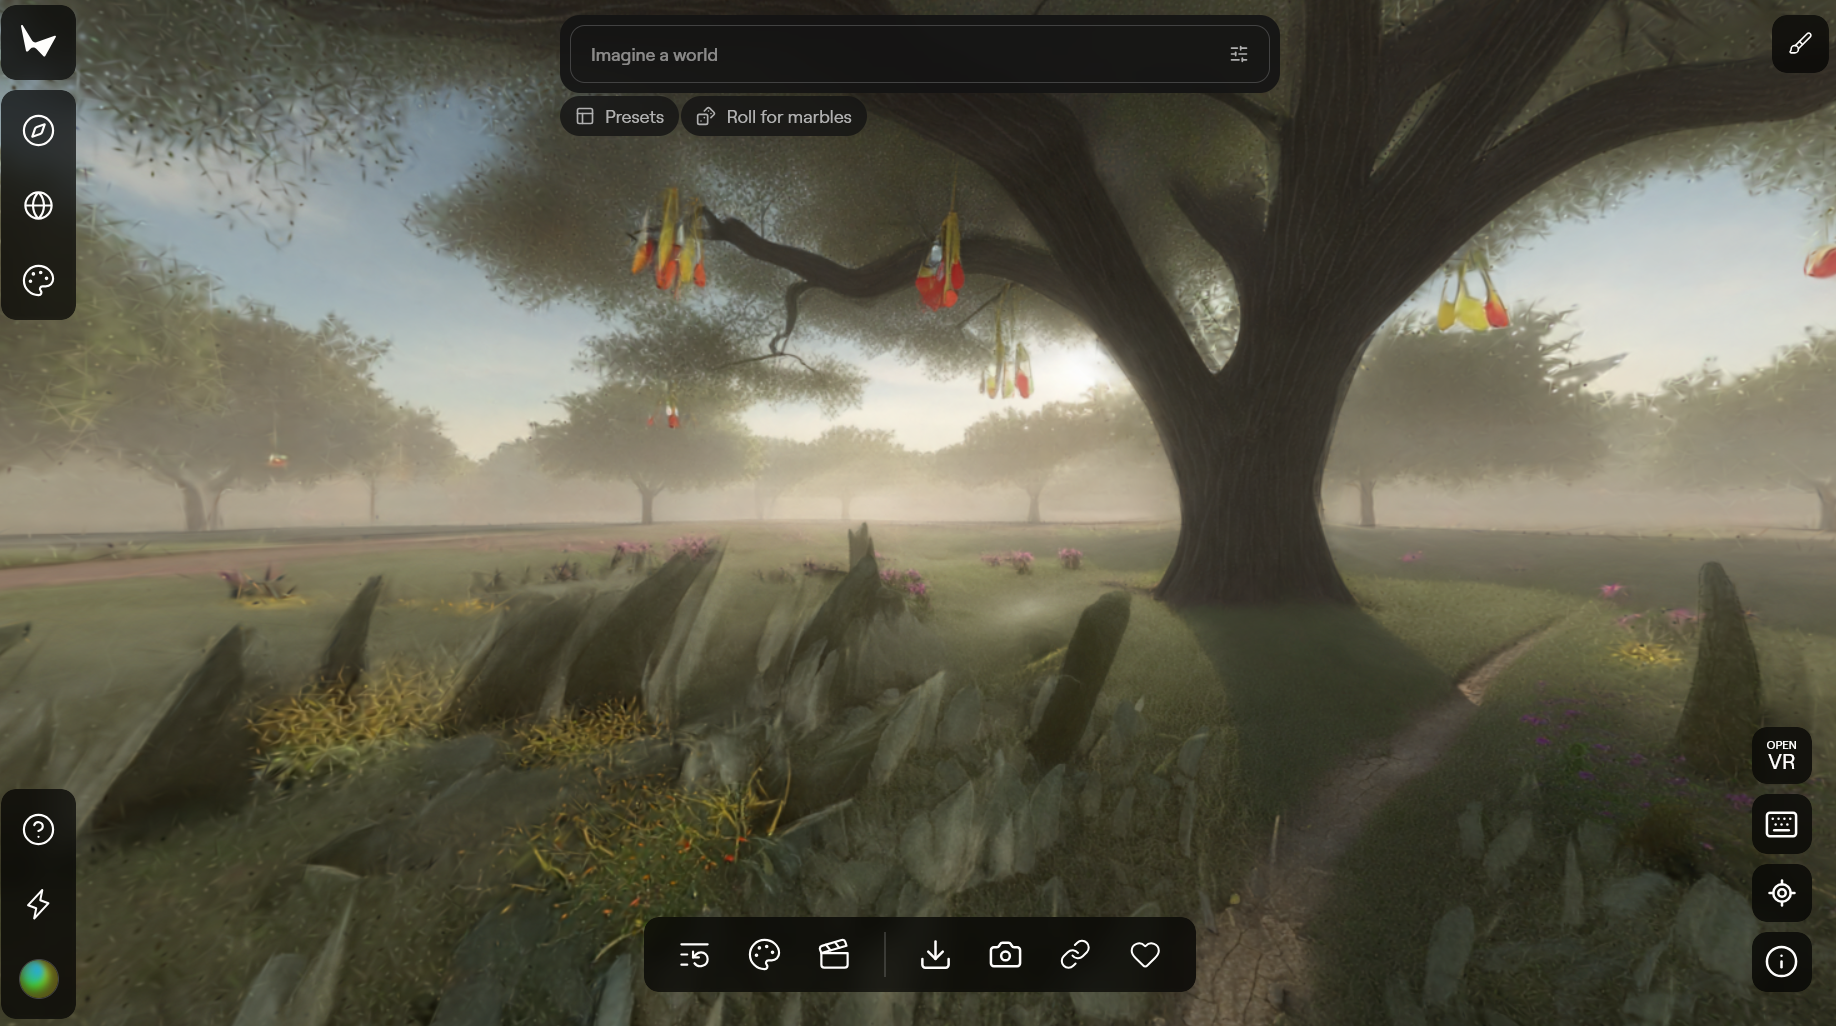
\includegraphics[width=0.9\textwidth,keepaspectratio]{images/mufasa_savana.png}
\caption{Caso Mufasa: Transizione verso la Gratitudine.}
\label{fig:marble_screenshots_mufasa}
\end{figure}

\begin{figure}[H]
\centering
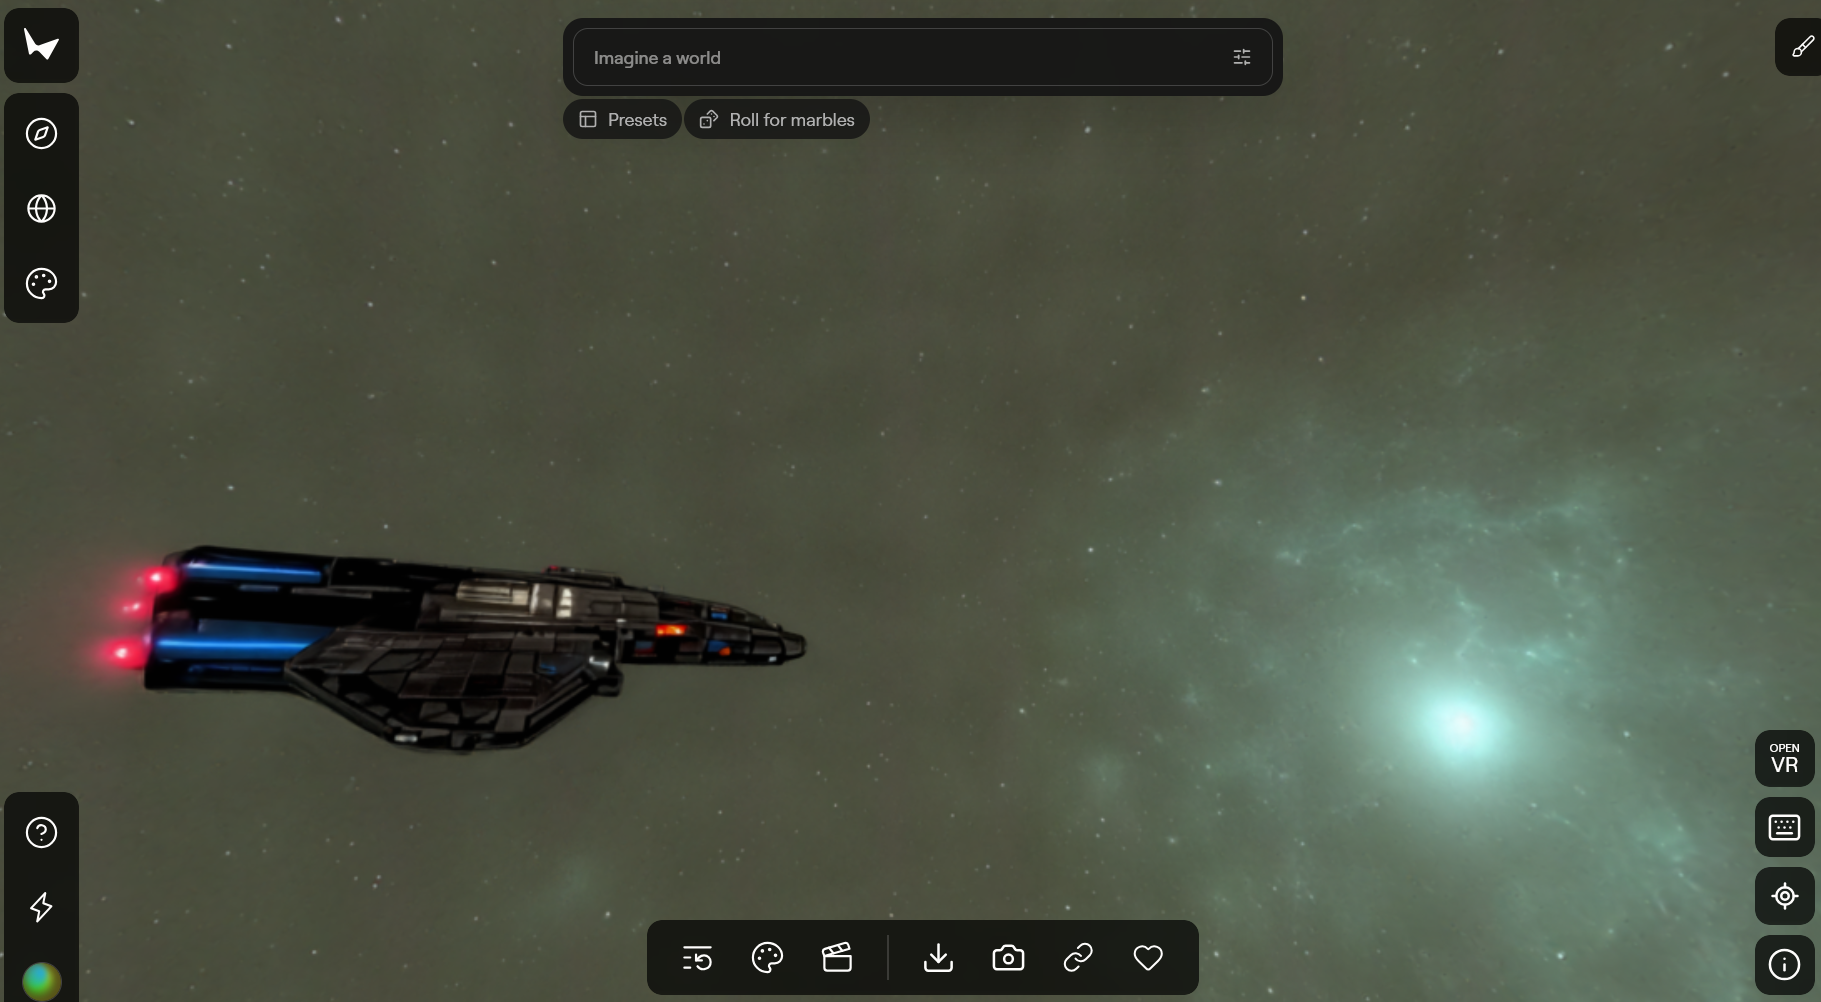
\includegraphics[width=0.9\textwidth,keepaspectratio]{images/prompt_031.png}
\caption{Caso Interstellar: Transizione verso la Speranza.}
\label{fig:marble_screenshots_interstellar}
\end{figure}

\subsection{Analisi Critica dei Risultati}
Sebbene la pipeline logico-affettiva funzioni correttamente nell'isolare i vettori emotivi e nel generare i relativi prompt descrittivi, la resa estetica finale all'interno del mondo \textit{Marble} evidenzia forti limiti strutturali, rendendo i risultati visivi non pienamente soddisfacenti per i seguenti motivi:

\begin{itemize}
    \item \textbf{Incoerenza Atmosferica e Cromatica (Caso Mufasa):} L'ambiente tridimensionale generato mostra una netta contraddizione visiva. A fronte di una marcata illuminazione zenitale sullo sfondo che suggerirebbe un'atmosfera calda e serena, il primo piano è dominato da una nebbia densa e da palette cromatiche fredde e sature. Inoltre, l'algoritmo di posizionamento degli asset ha introdotto artefatti visivi sulla vegetazione (elementi geometrici dai colori primari innaturali appesi alla chioma dell'albero) che compromettono l'armonia e il realismo della scena.
    \item \textbf{Povertà Scenica e Mancanza di Profondità (Caso Interstellar):} Nel secondo scenario, l'output si riduce alla renderizzazione di un singolo asset isolato (una navicella spaziale) inserito su una texture di sfondo bidimensionale e generica. Manca completamente una composizione geometrica complessa, un gioco di volumi o un'interazione tra luci e ombre che possa dare profondità alla scena e supportare visivamente il cambio di stato emotivo richiesto; elementi presenti nel prompt marble.
    \item \textbf{Limiti del Motore di Generazione Procedurale:} Le problematiche riscontrate evidenziano la rigidità del generatore interno di \textit{Marble}. Il sistema fatica a interpretare le sfumature semantiche e la complessità dei prompt forniti dall'LLM, tendendo ad appiattire l'output visivo. Il risultato è una disposizione caotica di asset preconfigurati o, al contrario, una scena eccessivamente spoglia, frammentando l'efficacia dell'esperienza liminale.
\end{itemize}
 
% ═══════════════════════════════════════════════════════════════════
%              CAPITOLO III - PROBLEMI CRITICI E SOLUZIONI
% ═══════════════════════════════════════════════════════════════════
\chapter{Problemi critici e soluzioni}
\label{ch:problemi}
 
\section{Tunnel SSH instabile $\rightarrow$ keepalive}
 

Il server chiude la connessione SSH dopo $\sim$51 secondi di inattività durante l'attesa della risposta di Llama. Gli appelli successivi falliscono con ``SSH session not active''.

 
La soluzione è stata l'aggiunta di \texttt{set\_keepalive=10} su \texttt{SSHTunnelForwarder} e 
transport.set\_keepalive(10) sul client Paramiko. Un segnale viene inviato ogni 10 secondi per mantenere la connessione attiva.

 

\begin{figure}[H]
\begin{verbatim}
tunnel = SSHTunnelForwarder(
    (hostname, port),
    ssh_username=user,
    ssh_password=password,
    remote_bind_address=(remote_host, remote_port),
    local_bind_address=("127.0.0.1", local_port),
    set_keepalive=10,  # keepalive ogni 10s
)
\end{verbatim}
\caption{Implementazione del keepalive SSH.}
\end{figure} 
 
\section{Tunnel SSH multipli $\rightarrow$ tunnel unico in \texttt{pipeline.py}}
 
Ogni modulo (\texttt{emotion\_fusion}, \texttt{cardinal\_point}, \texttt{build\_marble\_prompt}) apriva e chiudeva il proprio tunnel SSH indipendentemente, causando instabilità e conflitti di porta.

 
Adesso \texttt{pipeline.py} apre il tunnel \textbf{una sola volta} con \texttt{async with vpn\_tunnel()}, e tutti i moduli chiamano Llama direttamente su \texttt{localhost:11434} senza gestire la connessione.
 
 
\section{Porta 11434 occupata da Ollama locale}
 
Ollama in esecuzione locale occupa la porta 11434, impedendo al tunnel SSH di utilizzare la stessa porta per il redirect.
 
La soluzione sarebbe di chiudere Ollama locale (clic destro sull'icona $\rightarrow$ Quit Ollama) quando si utilizza il server remoto.
 
 
\section{Qwen3:1.7b troppo piccolo $\rightarrow$ Llama3 (8B)}
 
Qwen3:1.7b restituisce JSON vuoti per l'analisi emozionale del testo. Il modello non ha sufficiente capacità per classificare emozioni in italiano.

 
Utilizzo di Llama3 (8B) che produce classificazioni emozionali affidabili. Il modello è determinante per la qualità dell'intera pipeline: un modello insufficiente provoca errori a cascata nelle fasi successive.
 
\section{\texttt{asyncio.run()} annidato in \texttt{cardinal\_point.py}}
 
\texttt{cardinal\_point.py} chiamava \texttt{asyncio.run()} internamente, ma \texttt{pipeline.py} aveva già un event loop attivo per il tunnel SSH. Python non permette loop asincroni annidati.

 
la soluzione è stato di Rendere \texttt{cardinal\_point.py} completamente sincrono: \texttt{get\_emotion\_target()} diventa una funzione normale che chiama \texttt{call\_llama()} direttamente. La gestione asincrona è delegata esclusivamente a \texttt{pipeline.py}.
 
 
% ═══════════════════════════════════════════════════════════════════
%              CAPITOLO IV - RISULTATI E ANALISI
% ═══════════════════════════════════════════════════════════════════
\chapter{Risultati e analisi}
\label{ch:risultati}
 
\section{Casi benchmark testati}
 
\begin{longtable}{llll}
    \caption{Riepilogo dei casi benchmark con emozione dominante e punto cardinale.} \label{tab:benchmark} \\
    \toprule
    \textbf{Caso} & \textbf{Stimolo} & \textbf{Emozione dom.} & \textbf{Punto cardinale} \\
    \midrule
    \endfirsthead
    \toprule
    \textbf{Caso} & \textbf{Stimolo} & \textbf{Emozione dom.} & \textbf{Punto cardinale} \\
    \midrule
    \endhead
    case\_001 & Morte di Mufasa & Happy & perdita $\rightarrow$ gratitudine \\
    case\_002 & Wall-E ed EVE & Tenderness & solitudine $\rightarrow$ connessione \\
    case\_003 & Italia ai mondiali & Sad & delusione $\rightarrow$ riscatto \\
    case\_004 & ... & ... & ... \\
    case\_005 & ... & ... & ... \\
    % aggiungere gli altri casi
    \bottomrule
\end{longtable}
 
 
\section{Qualità dei prompt Marble}
 
% ── Tabella scores ──
\begin{table}[H]
    \centering
    \caption{Punteggi di valutazione per i casi benchmark (scala 1--5).}
    \label{tab:scores}
    \begin{tabular}{lccc}
        \toprule
        \textbf{Caso} & \textbf{Emotion align.} & \textbf{Cardinal align.} & \textbf{Media} \\
        \midrule
        case\_001 & -- & -- & -- \\
        case\_002 & -- & -- & -- \\
        case\_003 & -- & -- & -- \\
        % riempire con i risultati
        \midrule
        \textbf{Media} & -- & -- & -- \\
        \bottomrule
    \end{tabular}
\end{table}

 
\section{Limiti identificati}
 
\begin{enumerate}
    \item \textbf{Sensibilità al modello LLM}: la qualità dell'intera pipeline dipende dalla capacità del modello. Un modello insufficiente degrada tutte le fasi.
    \item \textbf{LLM-as-judge}: Llama valuta i propri output, introducendo un bias di autocompiacimento.
    \item \textbf{Interfaccia Marble manuale}: l'assenza di un'API richiede il copia-incolla manuale dei prompt.
     \item \textbf{interpretabilità del prompt da Marble}: a volte nonostante il prompt ben generato con specificità liminal, marble non riproduce il monde fedele alla descrizione.

\end{enumerate}
 
 
% ═══════════════════════════════════════════════════════════════════
%              CAPITOLO V - CONCLUSIONE
% ═══════════════════════════════════════════════════════════════════
\chapter{Conclusione}
\label{ch:conclusione}
 
questo progetto ha realizzato una pipeline funzionante end-to-end che trasforma dati emozionali multimodali (priming facciale, emozione realtime, messaggio testuale) in prompt narrativi per la generazione di mondi 3D in Marble. Il sistema integra con successo il quadro teorico del Liminal Design, utilizzando il concetto di punto cardinale per guidare la trasformazione emotiva dell'utente attraverso ambienti 3D esplorabili.
 
La pipeline si compone di sette fasi modulari, con quattro appelli a Llama che gestiscono le operazioni più complesse (analisi testuale, identificazione del punto cardinale, generazione del prompt, valutazione). L'architettura permette l'esecuzione sia in locale che su server remoto tramite tunnel SSH configurabile.
 
\subsection*{Contributi principali}
\begin{itemize}
    \item Pipeline modulare Python con fusione emozionale ponderata a tre segnali.
    \item Meta-prompt engineering con tabella emozione $\rightarrow$ mondo 3D e regole di trasformazione.
    \item Sistema di valutazione automatica LLM-as-judge con confronto progressivo.
    \item Infrastruttura dual-mode (locale/remoto) con tunnel SSH e keepalive.
\end{itemize}
 
\subsection*{Prossimi passi}
\begin{itemize}
    \item Integrazione diretta con FaceReader/Noldus per l'acquisizione delle emozioni in tempo reale.
    \item Sviluppo di un'API per Marble per automatizzare la generazione dei mondi.
    \item Valutazione umana dei prompt e dei mondi generati per validare i punteggi LLM-as-judge.
    \item Test con un modello LLM più grande (Llama3:70B) per migliorare la qualità dei prompt.
    \item interfacciamento se possibile nel futuro, lavorare con un generatore di mondo più efficiente.
\end{itemize}
 
 
% ═══════════════════════════════════════════════════════════════════
%                          APPENDICI
% ═══════════════════════════════════════════════════════════════════
\begin{appendices}
\titleformat{\chapter}[display]
  {\centering \normalfont\LARGE\bfseries}
  {Appendice \thechapter}
  {0.5ex}
  {\vspace{0.5ex}}

    \chapter{Meta-prompt completo}
    \label{app:metaprompt}
    
    \lstinputlisting[style=promptstyle, caption={Contenuto completo di meta\_prompt\_v2.txt.}]{codefiles/meta_prompt_v2.txt}
    
    \chapter{Tabella di mappatura emozione $\rightarrow$ mondo 3D}
    \label{app:emotion_map}
    
    \begin{table}[H]
        \centering
        \caption{Mappatura completa emozione $\rightarrow$ elementi del mondo Marble.}
        \footnotesize
        \begin{tabularx}{\textwidth}{l X X X}
            \toprule
            \textbf{Emozione} & \textbf{Ambiente} & \textbf{Colori} & \textbf{Elementi} \\
            \midrule
            Happy & Paesaggio aperto, giardino, savana & Giallo, oro, arancio, verde & Percorsi luminosi, particelle \\
            Tenderness & Spazio protetto, luce soffusa & Rosa, crema, azzurro & Lanterne, cuscini, curve \\
            Sad & Paesaggio sospeso, lago, nebbia & Blu, grigio, viola, argento & Acqua calma, stelle distanti \\
            Fear & Spazio protetto in ambiente incerto & Blu scuro, verde smorzato & Cupole, rifugi, porte aperte \\
            Anger & Paesaggio roccioso o metallico & Rosso, arancio, nero, rame & Fratture, lava controllata, vento \\
            Neutral & Spazio contemplativo minimale & Beige, grigio, azzurro pallido & Architettura semplice, acqua \\
            Surprise & Mondo rivelatorio, canyon, portale & Turchese, oro, viola, bianco & Portali, scale, costellazioni \\
            Disgust & Ambiente di purificazione & Verde scuro, grigio, bianco & Acqua, vapore, superfici pulite \\
            \bottomrule
        \end{tabularx}
    \end{table}
    
    
    \chapter{Esempi completi dei casi benchmark}
    \label{app:cases}
    
    % Inserire i 10+ casi completi con input JSON e output generato
    % Per ogni caso: stimulus, priming, realtime, message, fusion, cardinal, marble_prompt
    
    \begin{notabox}[Caso 001 - Morte di Mufasa]
    \textbf{Stimolo:} Death of Mufasa --- The Lion King \\
    \textbf{Emozione dominante:} Happy (score: 0.6375) \\
    \textbf{Punto cardinale:} dalla perdita alla presenza e gratitudine \\
    \textbf{Prompt Marble:} ``Imagine a sunlit savannah at dawn, where golden grasses sway gently in the morning breeze...''
    \end{notabox}
    

    
    
    \chapter{Guida all'installazione e riproduzione}
    \label{app:install}
    
    \begin{enumerate}
        \item Clonare il repository:
        \begin{lstlisting}[style=pythonstyle]
    git clone https://github.com/toyemryan/progetto_d22_marble.git
    cd progetto_d22_marble
        \end{lstlisting}
        
        \item Creare l'ambiente virtuale e installare le dipendenze:
        \begin{lstlisting}[style=pythonstyle]
    python -m venv .venv
    .venv\Scripts\activate    # Windows
    pip install -r requirements.txt
        \end{lstlisting}
        
        \item Installare Ollama e scaricare il modello:
        \begin{lstlisting}[style=pythonstyle]
    # Scaricare da https://ollama.com/download
    ollama pull llama3
    ollama pull qwen3:1.7b
        \end{lstlisting}
        
        \item Configurare il file \texttt{.env}:
        \begin{lstlisting}[style=pythonstyle]
    OLLAMA_URL=http://localhost:11434/api/generate
    OLLAMA_MODEL=llama3
    CONNECT_TO_REMOTE=false
        \end{lstlisting}
        
        \item Eseguire la pipeline:
        \begin{lstlisting}[style=pythonstyle]
    python src/pipeline.py --new       # nuovo caso interattivo
    python src/pipeline.py --last      # ultimo caso
    python src/pipeline.py --all       # tutti i casi
    python src/pipeline.py --evaluate  # valutazione
        \end{lstlisting}
    \end{enumerate}


\end{appendices}

\bibliographystyle{ieeetr}
\bibliography{bibl} 
\end{document}
